\section{List Structure}
\label{sec:list}
\begin{frame}<beamer>
    \frametitle{Outline}
    \tableofcontents[currentsection]
\end{frame}

\begin{frame}[fragile]{Overview of List Structure}
\vspace{0.1in}
\begin{figure}
	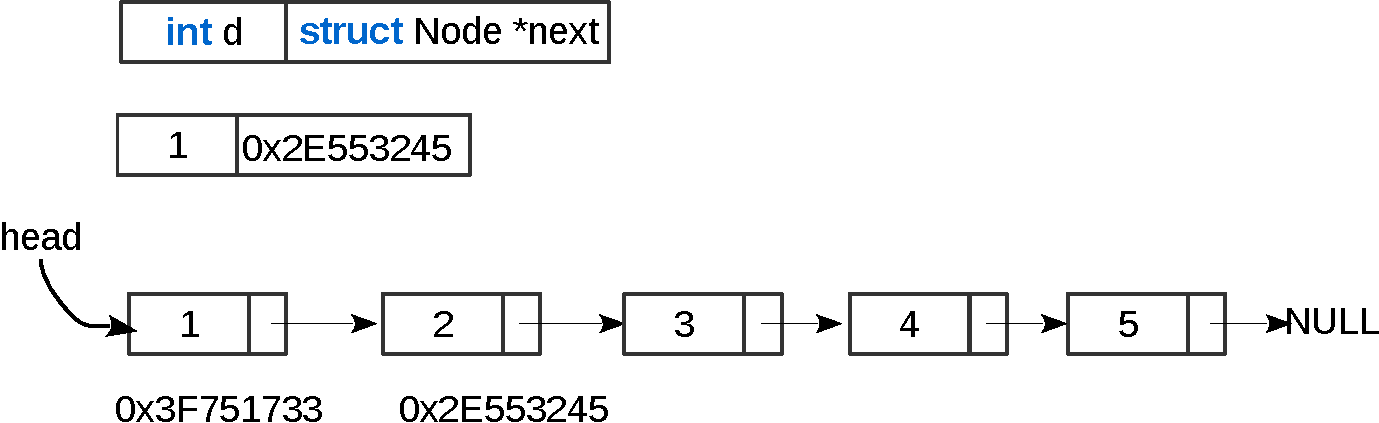
\includegraphics[width=0.8\linewidth]{figs/list.pdf}
\end{figure}
\begin{lstlisting}[xleftmargin=0.32\linewidth, linewidth=0.6\linewidth]
struct Node {
  int a;
  struct Node *next;
};
typedef Node TNode;
\end{lstlisting}
\end{frame}

\begin{frame}[fragile]{Build List---Step 1}
\begin{figure}
\begin{center}
	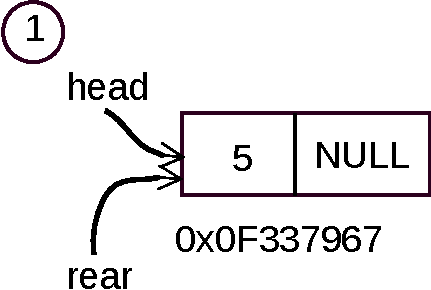
\includegraphics[width=0.25\linewidth]{figs/list_build_step1.pdf}
\end{center}
\end{figure}
\begin{lstlisting}[xleftmargin=0.05\linewidth, linewidth=0.9\linewidth]
struct Node {
  int a;
  struct Node *next;
};
typedef Node TNode;
int main()
{
  TNode *head = NULL, *rear = NULL;
  TNode *p = (TNode*)malloc(sizeof(TNode));
  p->a = 5; p->next = NULL;
  head = p; rear = p;
}
\end{lstlisting}
\end{frame}

\begin{frame}[fragile]{Build List---Step 2}
\vspace{-0.1in}
\begin{figure}
\begin{center}
	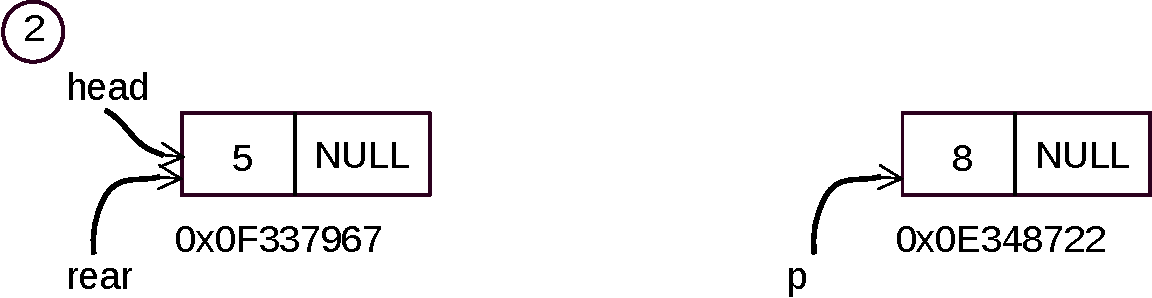
\includegraphics[width=0.55\linewidth]{figs/list_build_step2.pdf}
\end{center}
\end{figure}
\begin{lstlisting}[xleftmargin=0.05\linewidth, linewidth=0.9\linewidth]
struct Node {
  int a;
  struct Node *next;
};
typedef Node TNode;
TNode *buidList()
{
  TNode *head = NULL, *rear = NULL;
  TNode *p = (TNode*)malloc(sizeof(TNode));
  p->a = 5; p->next = NULL;
  head = p; rear = p;
  p = (TNode*)malloc(sizeof(TNode));
  return head;
}
\end{lstlisting}
\end{frame}

\begin{frame}[fragile]{Build List---Step 3}
\vspace{-0.1in}
\begin{figure}
\begin{center}
	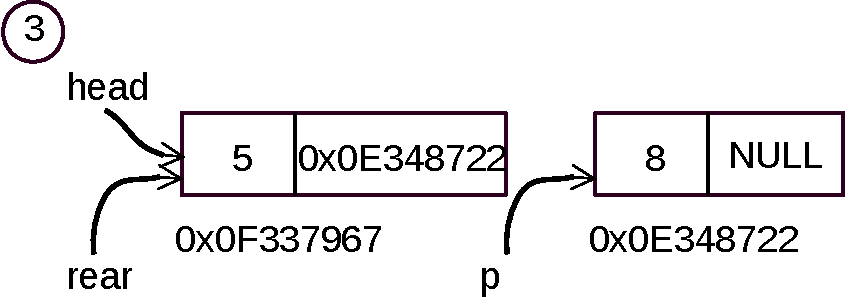
\includegraphics[width=0.5\linewidth]{figs/list_build_step3.pdf}
\end{center}
\end{figure}
\begin{lstlisting}[xleftmargin=0.05\linewidth, linewidth=0.9\linewidth]
TNode *buidList()
{
  TNode *head = NULL, *rear = NULL;
  TNode *p = (TNode*)malloc(sizeof(TNode));
  p->a = 5; p->next = NULL;
  head = p; rear = p;
  p = (TNode*)malloc(sizeof(TNode));
  rear->next = p;
  return head;
}
\end{lstlisting}
\end{frame}

\begin{frame}[fragile]{Build List---Step 4}
\vspace{-0.1in}
\begin{figure}
\begin{center}
	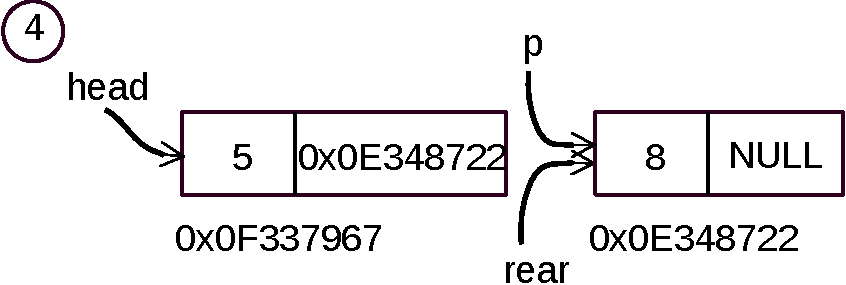
\includegraphics[width=0.5\linewidth]{figs/list_build_step4.pdf}
\end{center}
\end{figure}
\begin{lstlisting}[xleftmargin=0.05\linewidth, linewidth=0.9\linewidth]
TNode *buidList()
{
  TNode *head = NULL, *rear = NULL;
  TNode *p = (TNode*)malloc(sizeof(TNode));
  p->a = 5; p->next = NULL;
  head = p; rear = p;
  p = (TNode*)malloc(sizeof(TNode));
  rear->next = p;
  rear = p;
  return head;
}
\end{lstlisting}
\end{frame}

\begin{frame}[fragile]{Build List---Summary}
\vspace{-0.1in}
\begin{figure}
\begin{center}
	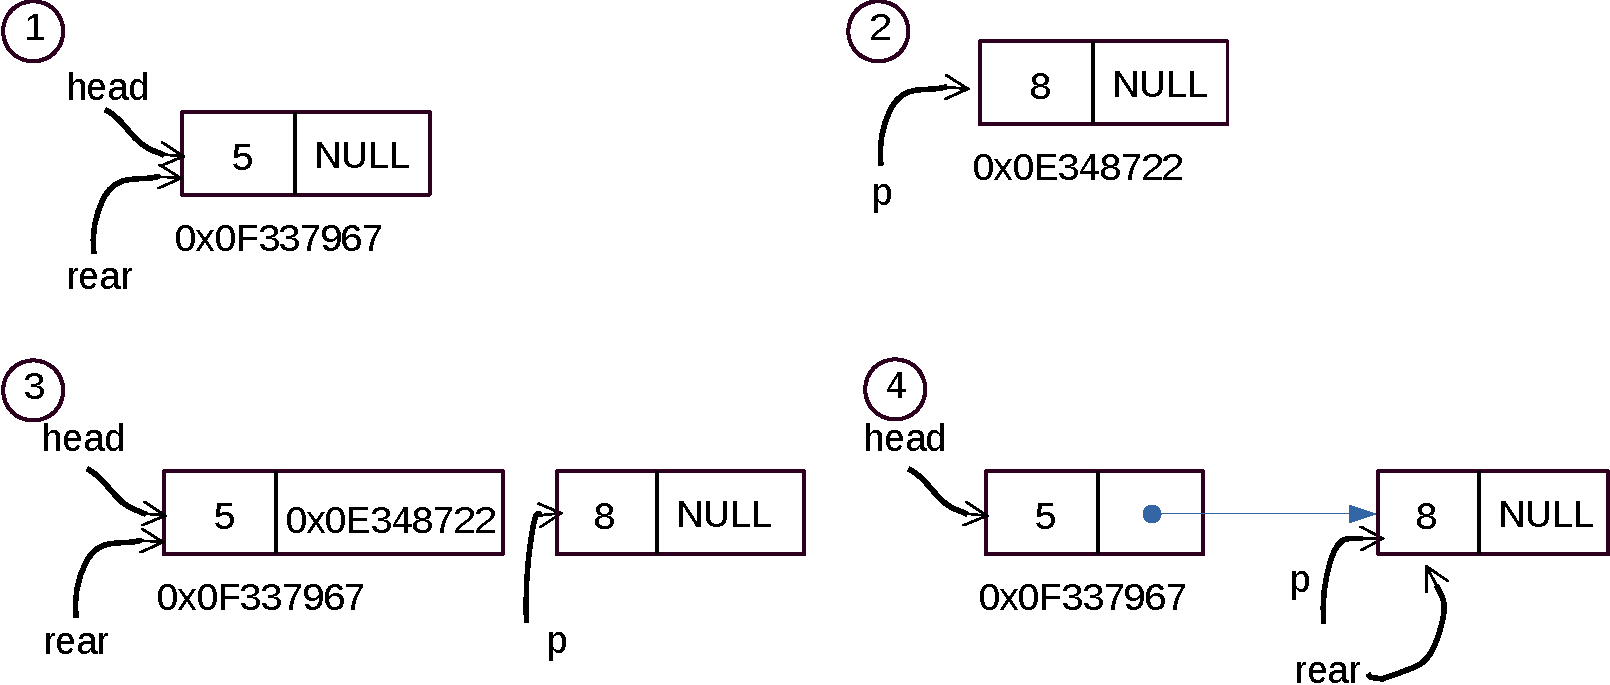
\includegraphics[width=0.85\linewidth]{figs/list_build.pdf}
\end{center}
\end{figure}
\end{frame}

\begin{frame}[fragile]{Print List}
\vspace{-0.1in}
\begin{figure}
\begin{center}
	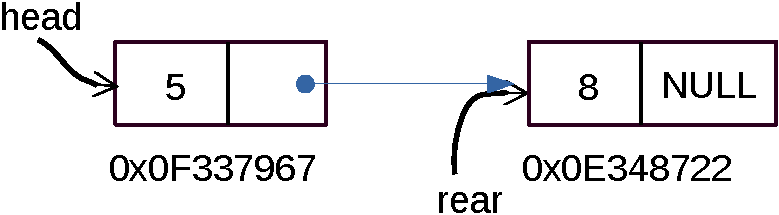
\includegraphics[width=0.4\linewidth]{figs/list_print.pdf}
\end{center}
\end{figure}
\begin{lstlisting}[xleftmargin=0.05\linewidth, linewidth=0.9\linewidth]
int printList(TNode *head)
{
  TNode *p = head;
  int i = 0;
  while(p != NULL)
  {
      printf("%3d\n", p->a);
      p = p->next;
      i++;
  }
  return i;
}
\end{lstlisting}
\end{frame}

\begin{frame}[fragile]{Delete Node from List}
\vspace{0.2in}
\begin{figure}
\begin{center}
	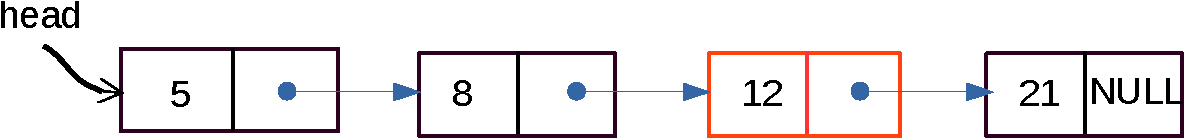
\includegraphics[width=0.6\linewidth]{figs/list_delete_step1.pdf}
\end{center}
\end{figure}
\begin{itemize}
	\item {We want to delete the node in which \textcolor{red}{a} equals to \textcolor{red}{12}}
\end{itemize}

\end{frame}

\begin{frame}[fragile]{Delete Node from List--Steps}
\begin{figure}
\begin{center}
	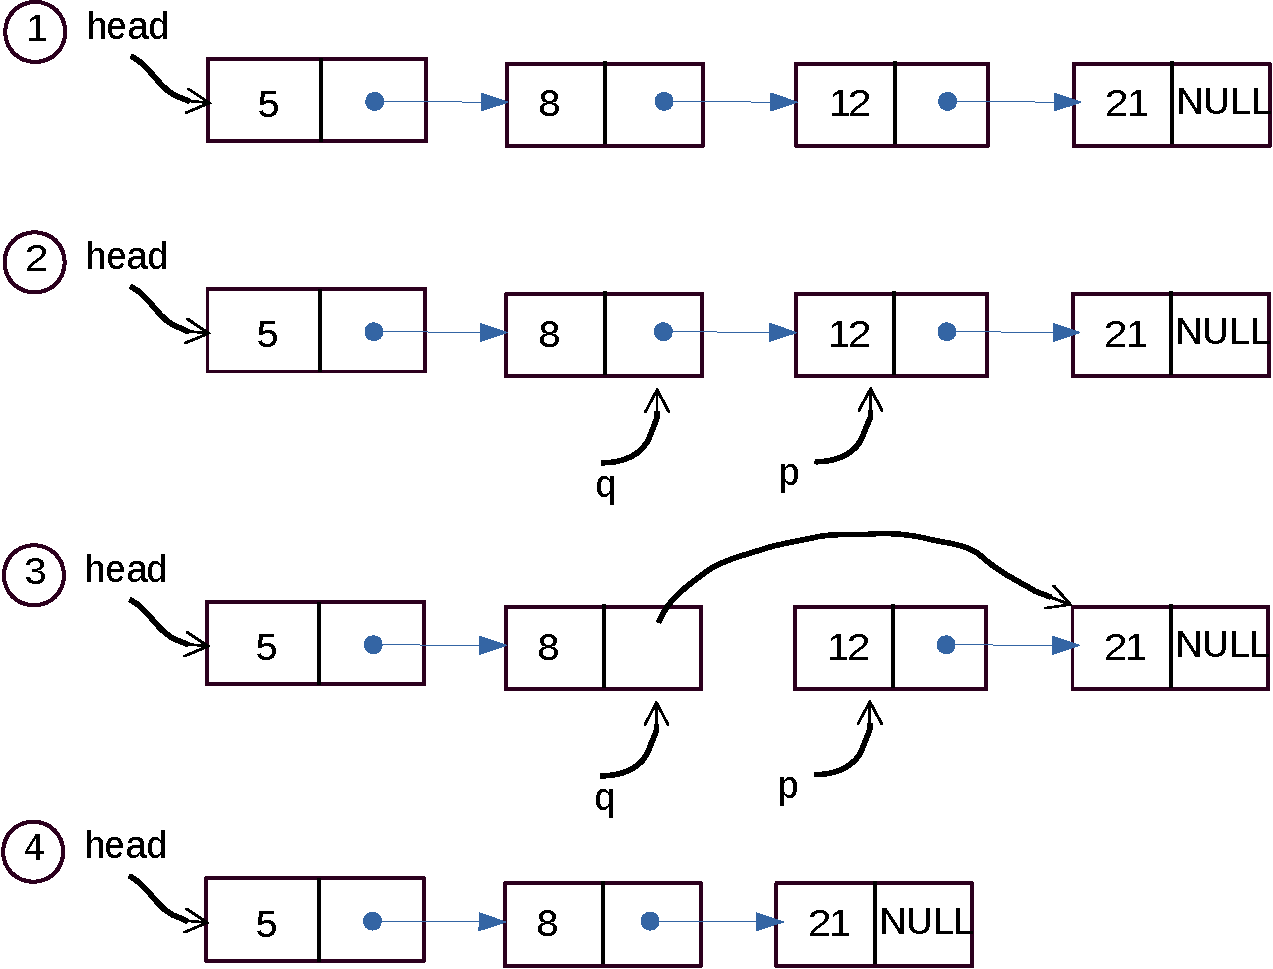
\includegraphics[width=0.75\linewidth]{figs/list_delete.pdf}
\end{center}
\end{figure}

\end{frame}

\begin{frame}[fragile]{Delete Node from List---Procedure}
\vspace{0.2in}
\begin{figure}
\begin{center}
	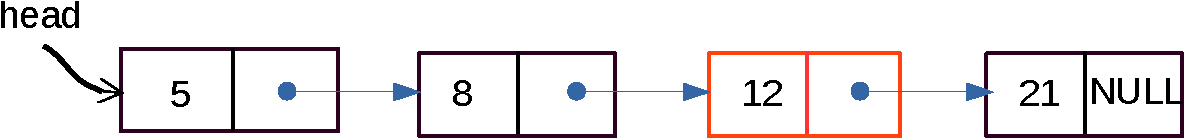
\includegraphics[width=0.6\linewidth]{figs/list_delete_step1.pdf}
\end{center}
\end{figure}
\begin{itemize}
	\item {We want to delete the node in which \textcolor{red}{a} equals to \textcolor{red}{12}}
\end{itemize}
\begin{enumerate}
	\item {Find the node, whose \textcolor{red}{a} equals to \textcolor{red}{12}}
	\item {Given it is \textcolor{red}{p}, the node before it is \textcolor{red}{q}}
	\begin{enumerate}
		\item {\mbox{q$->$next} = \mbox{p$->$next};}
		\item {p$->$next = NULL;}
		\item {free(p);}
	\end{enumerate}
\end{enumerate}

\end{frame}


\begin{frame}[fragile]{Delete Node from List---Codes}
\vspace{-0.1in}
\begin{figure}
\begin{center}
	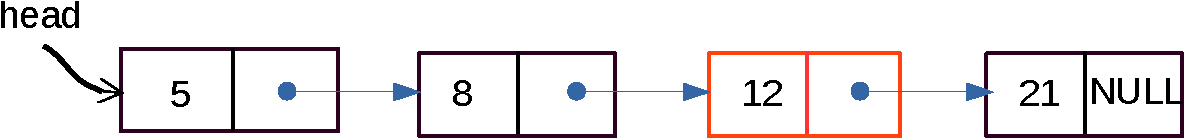
\includegraphics[width=0.6\linewidth]{figs/list_delete_step1.pdf}
\end{center}
\end{figure}
\begin{lstlisting}[xleftmargin=0.05\linewidth, linewidth=0.9\linewidth]
void deleteNode(int val, TNode *head)
{
   TNode *p = head, *q = head;
   //filling the codes here
}
\end{lstlisting}
\end{frame}

\begin{frame}[fragile]{Delete Node from List---The answer}
\vspace{-0.1in}
\begin{figure}
\begin{center}
	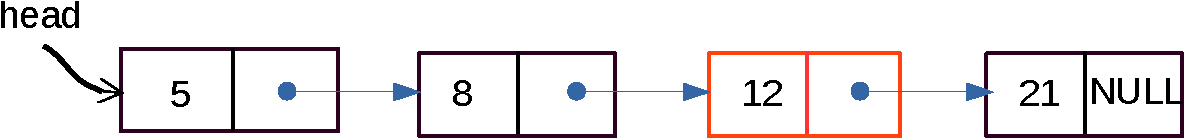
\includegraphics[width=0.6\linewidth]{figs/list_delete_step1.pdf}
\end{center}
\end{figure}
\begin{lstlisting}[xleftmargin=0.05\linewidth, linewidth=0.9\linewidth]
void deleteNode(int val, TNode *head)
{
   TNode *p = head, *q = head;
   while(p != NUL && p->a != val)
   {
       q = p;
       p = p->next;
   }
   if(p != NULL && p->a == val)
   {
       q->next = p->next;
       p->next = NULL;
       free(p);
   }
}
\end{lstlisting}
\vspace{-0.2in}
\textcolor{red}{Why condition ``p $!=$ NUL'' first???}
\end{frame}

\begin{frame}{What are the differences between Array and List}

\begin{table}
\begin{center}
\begin{tabular}{|l|c|c|} \hline
 & Array & List \\ \hline \hline
 Structure & linear & linear \\\hline
Memory & continous block & chain of blocks\\\hline
Visit & subscript & linear scan \\ \hline
Insert/delete & element shifting & direct  operation \\\hline\hline
\end{tabular}
\end{center}
\end{table}

\end{frame}